\documentclass[12pt,a4paper]{article}
\usepackage[utf8]{vietnam}
\usepackage{amsmath,amssymb}
\usepackage{tabularx}
\usepackage{tikz}
\usetikzlibrary{calc,angles,quotes,arrows.meta,patterns}
\usepackage{xcolor}
\usepackage{enumitem}
\usepackage{fancyhdr}
\usepackage[top=1.2cm, bottom=1.2cm, left=1.5cm, right=1.5cm]{geometry}
\usepackage[loigiai]{ex_test}
\SAOPTN{widthSA=2.6,heightSA=0.62}

\setlength{\headheight}{15pt}
\setlength{\parskip}{0pt}

\pagestyle{fancy}
\fancyhf{}
\rhead{\textit{Môn Toán 6 -- Hướng dẫn giải Đề số 2}}
\lhead{\textit{Bộ đề ôn tập Giữa học kì I}}
\cfoot{\thepage}

\begin{document}

\begin{center}
  \textbf{\Large HƯỚNG DẪN GIẢI CHI TIẾT VÀ BẢNG ĐÁP ÁN}\\
  \textbf{\large ĐỀ ÔN TẬP GIỮA HỌC KỲ I -- ĐỀ SỐ 2}\\
  \textit{Môn: Toán 6 -- Năm học 2026 -- 2027}
\end{center}
\vspace{2mm}

% --- BẢNG ĐÁP ÁN TRẮC NGHIỆM TỔNG HỢP ---
\noindent\textbf{\large A. BẢNG ĐÁP ÁN TRẮC NGHIỆM TỔNG HỢP}
\vspace{1.5mm}

\noindent\textbf{1. Phần I (Mỗi câu trả lời đúng được 0,25 điểm):}
\begin{center}
\begin{tabular}{|c|c|c|c|c|c|c|c|c|c|c|c|c|}
\hline
\textbf{Câu} & \textbf{1} & \textbf{2} & \textbf{3} & \textbf{4} & \textbf{5} & \textbf{6} & \textbf{7} & \textbf{8} & \textbf{9} & \textbf{10} & \textbf{11} & \textbf{12} \\
\hline
\textbf{Đ/A} & \textbf{C} & \textbf{A} & \textbf{C} & \textbf{D} & \textbf{C} & \textbf{B} & \textbf{A} & \textbf{D} & \textbf{C} & \textbf{A} & \textbf{D} & \textbf{C} \\
\hline
\end{tabular}
\end{center}
\vspace{1mm}

\noindent\textbf{2. Phần II (Đúng/Sai):}
\begin{center}
\begin{tabular}{|c|c|c|c|c||c|c|c|c|c|}
\hline
\textbf{Câu 1} & \textbf{a)} & \textbf{b)} & \textbf{c)} & \textbf{d)} & \textbf{Câu 2} & \textbf{a)} & \textbf{b)} & \textbf{c)} & \textbf{d)} \\
\hline
\textbf{Đ/S} & \textbf{S} & \textbf{S} & \textbf{Đ} & \textbf{S} & \textbf{Đ/S} & \textbf{Đ} & \textbf{S} & \textbf{S} & \textbf{S} \\
\hline
\end{tabular}
\end{center}
\vspace{1mm}

\noindent\textbf{3. Phần III (Mỗi câu trả lời đúng được 1,0 điểm):}
\begin{center}
\begin{tabular}{|c|c|c|}
\hline
\textbf{Câu} & \textbf{Câu 1} & \textbf{Câu 2} \\
\hline
\textbf{Đáp án} & \textbf{3} & \textbf{30} \\
\hline
\end{tabular}
\end{center}
\vspace{3mm}

% --- LỜI GIẢI CHI TIẾT ---
\noindent\textbf{\large B. HƯỚNG DẪN GIẢI CHI TIẾT TỪNG CÂU}
\vspace{2mm}

\noindent\textbf{\large PHẦN I. CÂU TRẮC NGHIỆM NHIỀU PHƯƠNG ÁN LỰA CHỌN}
\vspace{1mm}
\begin{ex}
Tập hợp các chữ cái trong cụm từ “CHĂM HỌC” là:
\choice
{$\{C; H; Ă; M; H; O; C\}$}
{$\{H; Ă; M; O\}$}
{\True $\{C; H; Ă; M; O\}$}
{$\{C; H; Ă; M; H; O\}$}
\loigiai{
Khi viết tập hợp các chữ cái của một từ, mỗi chữ cái chỉ viết một lần: $C, H, Ă, M, O$. Do đó tập hợp là $\{C; H; Ă; M; O\}$.
}
\end{ex}

\begin{ex}
Số tự nhiên liền sau của số $2022$ là:
\choice
{\True $2023$}
{$2020$}
{$2022$}
{$2024$}
\loigiai{
Số tự nhiên liền sau của $2022$ là $2022 + 1 = 2023$.
}
\end{ex}

\begin{ex}
Nếu $a \ \vdots \ 3$ và $b \ \vdots \ 3$ thì tổng $a + b$ chia hết cho:
\choice
{$0$}
{$6$}
{\True $3$}
{$9$}
\loigiai{
Theo tính chất chia hết của một tổng: Nếu các số hạng của một tổng đều chia hết cho cùng một số thì tổng chia hết cho số đó. Vì $a \ \vdots \ 3$ và $b \ \vdots \ 3$ nên $(a + b) \ \vdots \ 3$.
}
\end{ex}

\begin{ex}
Tổng nào sau đây chia hết cho $7$?
\choice
{$35 + 155 + 280$}
{$140 + 497 + 634$}
{$51 + 140 + 910$}
{\True $35 + 420 + 763$}
\loigiai{
Ta có: $35 = 7 \cdot 5 \ \vdots \ 7$, $420 = 7 \cdot 60 \ \vdots \ 7$, $763 = 7 \cdot 109 \ \vdots \ 7$. Do cả 3 số hạng đều chia hết cho 7 nên tổng $(35 + 420 + 763) \ \vdots \ 7$.
}
\end{ex}

\begin{ex}
Chọn khẳng định đúng trong các khẳng định sau:
\choice
{$4 < -5$}
{$2 < 0$}
{\True $0 > -3$}
{$-2 < -5$}
\loigiai{
Số 0 luôn lớn hơn mọi số nguyên âm, do đó $0 > -3$ là khẳng định đúng.
}
\end{ex}

\begin{ex}
Khẳng định nào dưới đây là đúng?
\choice
{Hình bình hành có bốn góc bằng nhau}
{\True Hình lục giác đều có 3 đường chéo chính cùng đi qua một điểm}
{Tam giác đều là tam giác có 3 góc vuông}
{Hình chữ nhật có hai đường chéo bằng nhau và vuông góc với nhau}
\loigiai{
Lục giác đều có 3 đường chéo chính cắt nhau tại trung điểm của mỗi đường và đi qua tâm đối xứng của lục giác.
}
\end{ex}

\begin{ex}
Cho tam giác đều $ABC$ có độ dài cạnh $AB = 7\text{ cm}$. Chu vi của tam giác $ABC$ là:
\choice
{\True $21\text{ cm}$}
{$49\text{ cm}$}
{$21\text{ cm}^2$}
{$49\text{ cm}^2$}
\loigiai{
Tam giác đều có 3 cạnh bằng nhau: $AB = BC = CA = 7\text{ cm}$. Chu vi tam giác $ABC$ là: $C = 3 \times 7 = 21\text{ cm}$.
}
\end{ex}

\begin{ex}
Hình nào sau đây không phải là lục giác đều?\begin{center}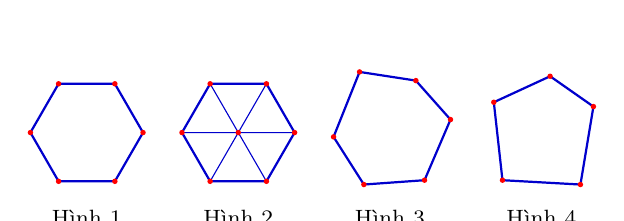
\begin{tikzpicture}[scale=0.55, line cap=round, line join=round]\begin{scope}[xshift=0cm]\foreach \i in {1,...,6} { \coordinate (P\i) at (\i*60:1.3); }\draw[thick, blue!80!black] (P1) -- (P2) -- (P3) -- (P4) -- (P5) -- (P6) -- cycle;\foreach \i in {1,...,6} { \fill[red] (P\i) circle (1.8pt); }\node[below=4pt, font=\footnotesize] at (0,-1.3) {Hình 1};\end{scope}\begin{scope}[xshift=3.5cm]\foreach \i in {1,...,6} { \coordinate (Q\i) at (\i*60:1.3); }\draw[thick, blue!80!black] (Q1) -- (Q2) -- (Q3) -- (Q4) -- (Q5) -- (Q6) -- cycle;\draw[blue!80!black] (Q1)--(Q4) (Q2)--(Q5) (Q3)--(Q6);\foreach \i in {1,...,6} { \fill[red] (Q\i) circle (1.8pt); }\fill[red] (0,0) circle (1.8pt);\node[below=4pt, font=\footnotesize] at (0,-1.3) {Hình 2};\end{scope}\begin{scope}[xshift=7cm]\coordinate (R1) at (1.4,0.3); \coordinate (R2) at (0.6,1.2); \coordinate (R3) at (-0.7,1.4);\coordinate (R4) at (-1.3,-0.1); \coordinate (R5) at (-0.6,-1.2); \coordinate (R6) at (0.8,-1.1);\draw[thick, blue!80!black] (R1) -- (R2) -- (R3) -- (R4) -- (R5) -- (R6) -- cycle;\foreach \p in {R1,R2,R3,R4,R5,R6} { \fill[red] (\p) circle (1.8pt); }\node[below=4pt, font=\footnotesize] at (0,-1.3) {Hình 3};\end{scope}\begin{scope}[xshift=10.5cm]\coordinate (S1) at (1.2,0.6); \coordinate (S2) at (0.2,1.3); \coordinate (S3) at (-1.1,0.7);\coordinate (S4) at (-0.9,-1.1); \coordinate (S5) at (0.9,-1.2);\draw[thick, blue!80!black] (S1) -- (S2) -- (S3) -- (S4) -- (S5) -- cycle;\foreach \p in {S1,S2,S3,S4,S5} { \fill[red] (\p) circle (1.8pt); }\node[below=4pt, font=\footnotesize] at (0,-1.3) {Hình 4};\end{scope}\end{tikzpicture}\end{center}
\choice
{Hình 3}
{Hình 2}
{Hình 1}
{\True Hình 4}
\loigiai{
Hình 4 là một ngũ giác (có 5 cạnh), không phải là lục giác đều.
}
\end{ex}

\begin{ex}
Chọn cách phân tích số $32$ ra thừa số nguyên tố đúng:
\choice
{$32 = 2 \cdot 16$}
{$32 = 8 \cdot 4$}
{\True $32 = 2^5$}
{$32 = 2 \cdot 4 \cdot 4$}
\loigiai{
Ta có: $32 = 2 \cdot 2 \cdot 2 \cdot 2 \cdot 2 = 2^5$. Các số 16, 8, 4 không phải là số nguyên tố.
}
\end{ex}

\begin{ex}
Trong các số sau, số nào chia hết cho cả $2$ và $5$?
\choice
{\True $2020$}
{$25$}
{$52$}
{$5$}
\loigiai{
Số chia hết cho cả 2 và 5 là số có chữ số tận cùng bằng 0. Trong các số trên, chỉ có số 2020 có tận cùng là 0.
}
\end{ex}

\begin{ex}
Trong các hình sau, hình nào có hai đường chéo không bằng nhau?
\choice
{Hình chữ nhật}
{Hình thang cân}
{Hình vuông}
{\True Hình bình hành}
\loigiai{
Hình chữ nhật, hình thang cân và hình vuông đều có hai đường chéo bằng nhau. Hình bình hành tổng quát có hai đường chéo cắt nhau tại trung điểm nhưng không bằng nhau.
}
\end{ex}

\begin{ex}
\immini{
Nếu có hai miếng bìa hình thang cân với kích thước như hình bên, ta ghép được hình nào sau đây?
\choice
{Hình vuông, hình chữ nhật}
{Hình vuông, hình bình hành}
{\True Hình bình hành, lục giác đều}
{Lục giác đều, hình thang cân}
}{
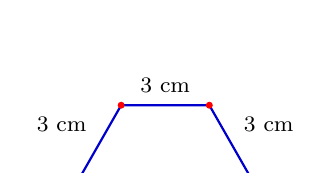
\begin{tikzpicture}[scale=0.7, baseline=(current bounding box.center), line cap=round, line join=round]
  \coordinate (A) at (0.8, 1.4); \coordinate (B) at (2.4, 1.4); \coordinate (C) at (3.2, 0); \coordinate (D) at (0, 0);
  \draw[thick, blue!80!black] (A) -- (B) -- (C) -- (D) -- cycle;
  \foreach \p in {A,B,C,D} \fill[red] (\p) circle (1.8pt);
  \node[above=1pt, font=\footnotesize] at (1.6, 1.4) {$3\text{ cm}$};
  \node[above left=1pt, font=\footnotesize] at (0.4, 0.7) {$3\text{ cm}$};
  \node[above right=1pt, font=\footnotesize] at (2.8, 0.7) {$3\text{ cm}$};
\end{tikzpicture}
}
\loigiai{
Ghép hai hình thang cân bằng nhau theo đáy lớn chung ta được hình lục giác đều (nếu đáy lớn gấp đôi đáy nhỏ) hoặc ghép đảo chiều ta được hình bình hành.
}
\end{ex}


\setcounter{ex}{0}
\noindent\textbf{\large PHẦN II. CÂU TRẮC NGHIỆM ĐÚNG SAI}
\vspace{1mm}
\begin{ex}
Xét trong $20$ số tự nhiên đầu tiên (từ $0$ đến $19$). Các khẳng định sau đây đúng hay sai?
\choiceTF
{Trong các số đã cho, có $3$ số chia hết cho cả $2$ và $5$}
{Trong các số đã cho, có $6$ số chia hết cho $9$}
{\True Trong các số đã cho, có $8$ số là số nguyên tố}
{Trong các số đã cho, có $6$ số là bội của $3$}
\loigiai{
\begin{itemize}[leftmargin=0.6cm, itemsep=1pt]
\item \textbf{a)} \textbf{Sai}. Các số chia hết cho cả 2 và 5 là số có tận cùng bằng 0: gồm $\{0; 10\}$ (chỉ có 2 số). Khẳng định sai.
\item \textbf{b)} \textbf{Sai}. Các số chia hết cho 9 từ 0 đến 19 gồm $\{0; 9; 18\}$ (chỉ có 3 số). Khẳng định sai.
\item \textbf{c)} \textbf{Đúng}. Các số nguyên tố từ 0 đến 19 gồm: $\{2; 3; 5; 7; 11; 13; 17; 19\}$ (đúng 8 số). Khẳng định đúng.
\item \textbf{d)} \textbf{Sai}. Các bội của 3 từ 0 đến 19 gồm: $\{0; 3; 6; 9; 12; 15; 18\}$ (có 7 số). Khẳng định sai.
\end{itemize}
}
\end{ex}

\begin{ex}
Xét việc phân tích số $40$ ra thừa số nguyên tố. Các khẳng định sau đây đúng hay sai?
\choiceTF
{\True Phân tích số $40$ ra thừa số nguyên tố ta được kết quả là $40 = 2^3 \cdot 5$}
{Kết quả phân tích số $40$ ra thừa số nguyên tố là $40 = 4 \cdot 10$}
{Kết quả phân tích số $40$ ra thừa số nguyên tố là $40 = 2 \cdot 4 \cdot 5$}
{Số $40$ có tất cả $3$ thừa số nguyên tố khác nhau là $2, 3$ và $5$}
\loigiai{
\begin{itemize}[leftmargin=0.6cm, itemsep=1pt]
\item \textbf{a)} \textbf{Đúng}. Ta có: $40 = 8 \cdot 5 = 2^3 \cdot 5$. Các thừa số 2 và 5 đều là số nguyên tố. Khẳng định đúng.
\item \textbf{b)} \textbf{Sai}. Các số 4 và 10 là hợp số, không phải thừa số nguyên tố. Khẳng định sai.
\item \textbf{c)} \textbf{Sai}. Số 4 là hợp số, chưa phân tích triệt để ra thừa số nguyên tố. Khẳng định sai.
\item \textbf{d)} \textbf{Sai}. Số 40 chỉ chia hết cho hai số nguyên tố là 2 và 5 (không chia hết cho 3). Khẳng định sai.
\end{itemize}
}
\end{ex}


\setcounter{ex}{0}
\noindent\textbf{\large PHẦN III. CÂU HỎI TRẢ LỜI NGẮN}
\vspace{1mm}
\begin{ex}
Có bao nhiêu số tự nhiên $m$ sao cho $5 < m < 15$ và $m \ \vdots \ 3$? \shortans{$3$}
\loigiai{
Các số tự nhiên lớn hơn 5 và nhỏ hơn 15 chia hết cho 3 là: $\{6; 9; 12\}$. Vậy có 3 số.
}
\end{ex}

\begin{ex}
Tìm số tự nhiên $x$ lớn nhất thỏa mãn $120 \ \vdots \ x$ và $150 \ \vdots \ x$. \shortans{$30$}
\loigiai{
Vì $x$ lớn nhất thỏa mãn $120 \ \vdots \ x$ và $150 \ \vdots \ x$ nên $x = \text{ƯCLN}(120, 150)$. Ta có: $120 = 2^3 \cdot 3 \cdot 5$; $150 = 2 \cdot 3 \cdot 5^2$. Do đó $\text{ƯCLN}(120, 150) = 2 \cdot 3 \cdot 5 = 30$. Vậy $x = 30$.
}
\end{ex}


\setcounter{ex}{0}
\noindent\textbf{\large PHẦN IV. TỰ LUẬN (3,0 ĐIỂM - CÓ BAREM ĐIỂM CHI TIẾT)}
\vspace{1mm}
\begin{ex} (1.0 điểm)
Thực hiện phép tính (tính hợp lí nếu có thể):
\begin{enumerate}[label=\textbf{\alph*)}, leftmargin=0.8cm, itemsep=2pt]
\item $3^4 : 3^2$
\item $80 - (4 \cdot 5^2 - 3 \cdot 2^3)$
\item $23 \cdot 75 + 25 \cdot 10 + 25 \cdot 13$
\end{enumerate}
\loigiai{
\begin{itemize}[leftmargin=0.5cm, itemsep=3pt]
\item \textbf{a)} $3^4 : 3^2 = 3^{4-2} = 3^2 = 9$. \hfill \textbf{[0.25đ]}
\item \textbf{b)} $80 - (4 \cdot 5^2 - 3 \cdot 2^3) = 80 - (4 \cdot 25 - 3 \cdot 8) = 80 - (100 - 24) = 80 - 76 = 4$. \hfill \textbf{[0.5đ]}
\item \textbf{c)} $23 \cdot 75 + 25 \cdot 10 + 25 \cdot 13 = 23 \cdot 75 + 25 \cdot (10 + 13) = 23 \cdot 75 + 25 \cdot 23 = 23 \cdot (75 + 25) = 23 \cdot 100 = 2300$. \hfill \textbf{[0.25đ]}
\end{itemize}
}
\end{ex}
\vspace{1.5mm}

\begin{ex} (0.75 điểm)
Tìm số tự nhiên $x$, biết:
\begin{enumerate}[label=\textbf{\alph*)}, leftmargin=0.8cm, itemsep=2pt]
\item $120 - 5(x + 2) = 20$
\item $x \ \vdots \ 20$, $x \ \vdots \ 35$ và $400 < x < 500$
\end{enumerate}
\loigiai{
\begin{itemize}[leftmargin=0.5cm, itemsep=3pt]
\item \textbf{a)} Ta có:\
$5(x + 2) = 120 - 20$\
$5(x + 2) = 100$\
$x + 2 = 100 : 5 = 20$\
$x = 20 - 2 = 18$. \hfill \textbf{[0.5đ]}
\item \textbf{b)} Vì $x \ \vdots \ 20$ và $x \ \vdots \ 35$ nên $x \in \text{BC}(20, 35)$.\
Ta có: $20 = 2^2 \cdot 5$; $35 = 5 \cdot 7 \implies \text{BCNN}(20, 35) = 2^2 \cdot 5 \cdot 7 = 140$.\
Suy ra $\text{BC}(20, 35) = \{0; 140; 280; 420; 560; \dots\}$.\
Vì $400 < x < 500$ nên $x = 420$. \hfill \textbf{[0.25đ]}
\end{itemize}
}
\end{ex}
\vspace{1.5mm}

\begin{ex} (0.75 điểm)
Cô giáo chủ nhiệm muốn chia $72$ quyển vở, $48$ bút bi và $60$ gói bánh thành một số phần thưởng như nhau để trao trong dịp sơ kết học kì.
\begin{enumerate}[label=\textbf{\alph*)}, leftmargin=0.8cm, itemsep=2pt]
\item Hỏi có thể chia được nhiều nhất bao nhiêu phần thưởng?
\item Khi đó mỗi phần thưởng có bao nhiêu quyển vở, bút bi và gói bánh?
\end{enumerate}
\loigiai{
\begin{itemize}[leftmargin=0.5cm, itemsep=3pt]
\item \textbf{a)} Gọi số phần thưởng nhiều nhất có thể chia được là $a$ ($a \in \mathbb{N}^*$).\
Theo đề bài: $72 \ \vdots \ a$, $48 \ \vdots \ a$, $60 \ \vdots \ a$ và $a$ lớn nhất nên $a = \text{ƯCLN}(72, 48, 60)$.\
Ta có: $72 = 2^3 \cdot 3^2$; $48 = 2^4 \cdot 3$; $60 = 2^2 \cdot 3 \cdot 5$.\
$\implies \text{ƯCLN}(72, 48, 60) = 2^2 \cdot 3 = 12$.\
Vậy có thể chia được nhiều nhất $12$ phần thưởng. \hfill \textbf{[0.5đ]}
\item \textbf{b)} Khi đó mỗi phần thưởng có:\
Số quyển vở: $72 : 12 = 6$ (quyển).\
Số bút bi: $48 : 12 = 4$ (bút).\
Số gói bánh: $60 : 12 = 5$ (gói). \hfill \textbf{[0.25đ]}
\end{itemize}
}
\end{ex}
\vspace{1.5mm}

\begin{ex} (0.5 điểm)
\begin{enumerate}[label=\textbf{\alph*)}, leftmargin=0.8cm, itemsep=2pt]
\item Cho số tự nhiên $x$ thỏa mãn $3^{x+1} + 3^{x+2} - 2 \cdot 3^x = 270$. Hỏi $x$ là số nguyên tố hay hợp số?
\item Tìm hai số tự nhiên biết tích của chúng bằng $144$ và ước chung lớn nhất của chúng bằng $6$.
\end{enumerate}
\loigiai{
\begin{itemize}[leftmargin=0.5cm, itemsep=3pt]
\item \textbf{a)} Ta có:\
$3^{x+1} + 3^{x+2} - 2 \cdot 3^x = 270$\
$3^x \cdot (3 + 9 - 2) = 270$\
$3^x \cdot 10 = 270$\
$3^x = 27 = 3^3 \implies x = 3$.\
Vì số $3$ chỉ có hai ước là 1 và chính nó nên $x = 3$ là số nguyên tố. \hfill \textbf{[0.25đ]}
\item \textbf{b)} Gọi hai số tự nhiên cần tìm là $u$ và $v$ ($u \le v$).\
Vì $\text{ƯCLN}(u, v) = 6$ nên đặt $u = 6m, v = 6n$ với $m, n \in \mathbb{N}^*$, $\text{ƯCLN}(m, n) = 1$ và $m \le n$.\
Theo đề bài: $u \cdot v = 144 \implies 6m \cdot 6n = 144 \implies 36mn = 144 \implies mn = 4$.\
Vì $\text{ƯCLN}(m, n) = 1$ và $m \le n$ nên ta chọn $m = 1, n = 4$.\
Suy ra: $u = 6 \cdot 1 = 6$ và $v = 6 \cdot 4 = 24$.\
Vậy hai số tự nhiên cần tìm là $6$ và $24$. \hfill \textbf{[0.25đ]}
\end{itemize}
}
\end{ex}
\vspace{1.5mm}


\begin{center}
\rule{4cm}{0.4pt}\\
\textit{--- HẾT ---}
\end{center}
\end{document}
